\section{System Design and Methods}

\subsection{System Overview and Division of Responsibilities}
Cloudra investigates reaction mechanisms by constructing candidate molecular configurations, locating and characterizing stationary points, tracing elementary reaction paths, and comparing competing channels under the specified reaction conditions and computational requirements. A workflow graph organizes tool calls and computational tasks by their execution dependencies. Cloudra's Delivery DAG represents the mechanism being delivered: its nodes are species occurrences, and its edges are elementary reaction steps. Agents must express candidate species and their reaction connections in this chemical graph. They choose subsequent geometric operations, calculations, and exploration branches from their hypotheses and returned results.

Canonical topology and stereochemical comparisons identify the species represented by a structure, while atom mapping identifies corresponding atoms across reactant and product configurations. Geometric operators rotate, translate, and assemble molecular fragments. Frequency calculations determine stationary-point curvature, and IRC calculations followed by endpoint optimization and frequency analysis determine which species a saddle point connects.

The Coordinator proposes mechanistic hypotheses and candidate elementary steps, and selects which branches to investigate. Computational agents prepare three-dimensional structures with the geometric operators and submit quantum-chemical calculations for their assigned steps. If a geometry diverges, a saddle-point optimization fails to converge, or a path bifurcates, the computational agent examines the structures and calculation diagnostics to decide whether to continue the step. If the step appears blocked, it reports the diagnosis to the Coordinator, which revises the hypothesis or explores another branch. The Supervisor reviews the species, steps, and calculation results in the DAG against the task requirements. Its review notes are stored separately from the facts parsed from calculation outputs.

\begin{figure*}[!tbp]
\centering
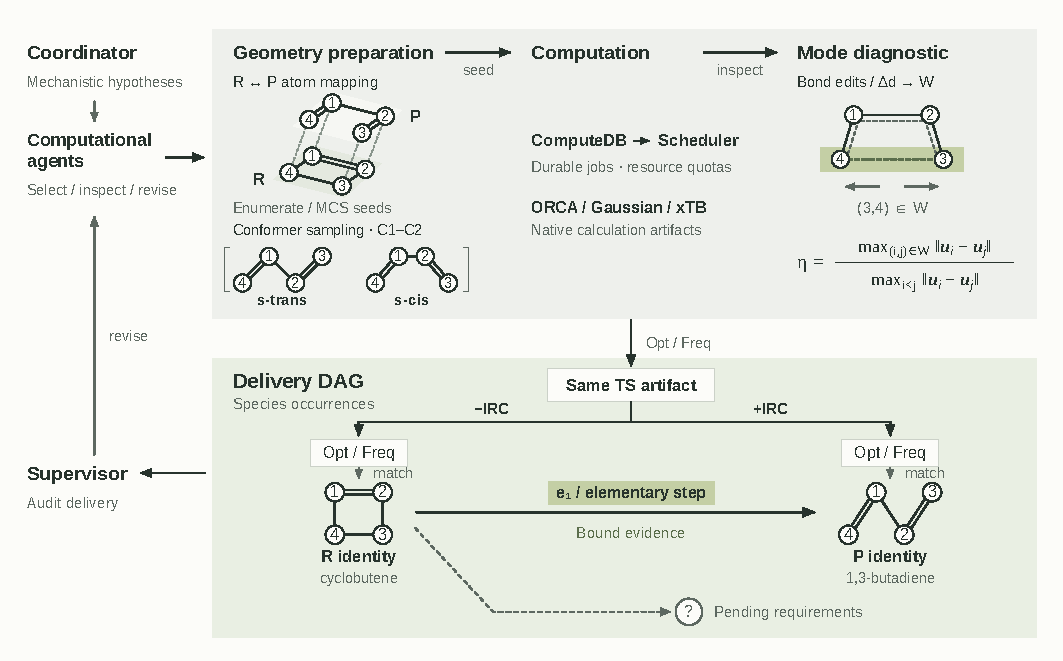
\includegraphics[width=\textwidth]{figures/Cloudra_Architecture_Stacked.pdf}
\caption{Cloudra's mechanism exploration workflow. Atom mapping and conformer sampling prepare reactant and product structures; ComputeDB and the scheduler manage the calculations. Mode diagnostics measure motion on monitored atom pairs. Bidirectional IRCs start from the same transition state, and their outer frames undergo endpoint optimization and frequency analysis. The resulting structures are compared with the species declared in the Delivery DAG. The Supervisor reviews the graph and identifies calculations to complete and assignments to resolve.}
\label{fig:04}
\end{figure*}

\subsubsection{Asynchronous Computation Scheduling and Resource Management}
The calculation database (\texttt{ComputeDB}) stores each job's status. Separate capacity pools limit concurrent calculations on local workers, remote SSH clusters, and Slurm queues. Before dispatch, the scheduler computes a SHA-256 digest from the Cartesian coordinates, spin, charge, and level of theory. The scheduler reuses a matching active job or cached result. Operating-system exclusive file locks (\texttt{flock}) track running processes and concurrency; quantum-chemistry processes holding active locks remain running during monitor exceptions. When a calculation ends, a scheduler notification triggers asynchronous output reading by the computational agent.

\subsection{Molecular Representations and Geometric Operators}
A molecular input consists of an attributed graph $H=(A,B)$ and Cartesian coordinates $\mathbf{X}\in\mathbb{R}^{n\times 3}$. Here $A$ is the atom set, $B$ is the bond set, and each row of $\mathbf{X}$ gives one atom position. The graph stores atom and bond attributes. Geometric operators change the coordinates and return measurements of the resulting structure. Replacing atoms or functional groups also changes $H$.

\subsubsection{Atom Correspondence and Reaction Centers}
Atom attributes retain element, isotope, formal charge, hydrogen count, radical-electron count, and declared stereochemistry; bond attributes retain order and stereochemical labels. Existing coordinates are retained. ETKDGv3 \citep{ref12,etkdg2020,ref13} embeds the remaining components, which are then assembled if necessary. Complete, unique atom-map labels on both endpoints define the correspondence directly and must agree in element and isotope. Otherwise, let $A_{\mathrm{P}}$ and $A_{\mathrm{R}}$ be the product and reactant heavy-atom sets. Candidate bijections $\pi:A_{\mathrm{P}}\to A_{\mathrm{R}}$ satisfy $z_i^{\mathrm{P}}=z_{\pi(i)}^{\mathrm{R}}$ and $\iota_i^{\mathrm{P}}=\iota_{\pi(i)}^{\mathrm{R}}$, where $z$ is atomic number and $\iota$ is isotope label. Each candidate is scored by

\begin{equation}\label{eq:methods-01}
\begin{aligned}
J(\pi)={}&2(N_{\mathrm{f}}+N_{\mathrm{b}})+N_{\mathrm{o}}\\
&+4\Delta_H+8\Delta_q+8\Delta_r+2N_{\mathrm{s}}.
\end{aligned}
\end{equation}

Let $B_{\mathrm{P}}^\pi$ denote product bonds expressed in reactant atom indices. Bond formation and cleavage are the set differences $B_{\mathrm{P}}^\pi\setminus B_{\mathrm{R}}$ and $B_{\mathrm{R}}\setminus B_{\mathrm{P}}^\pi$, with cardinalities $N_{\mathrm{f}}$ and $N_{\mathrm{b}}$. The count $N_{\mathrm{o}}$ includes pairs in $B_{\mathrm{P}}^\pi\cap B_{\mathrm{R}}$ whose bond orders differ. For $a\in\{H,q,r\}$, the mismatch is $\Delta_a=\sum_{i\in A_{\mathrm{P}}}|a_i^{\mathrm{P}}-a_{\pi(i)}^{\mathrm{R}}|$, where $H$, $q$, and $r$ are the atom hydrogen count, formal charge, and radical-electron count. $N_{\mathrm{s}}$ counts stereochemical mismatches. Exactly one declared tetrahedral label contributes one mismatch, increasing $J$ by 2. When both corresponding atoms carry tetrahedral labels, the comparison requires four corresponding neighbors, including a single hydrogen where applicable; it corrects for neighbor-order parity before comparing the labels. For two-sided labels, only comparable environments enter mismatch scoring.

For element–isotope classes of sizes $n_g$, the search space contains $N_\Pi=\prod_g n_g!$ bijections. All are enumerated when $N_\Pi\le 10^5$. Above this limit, MCS seeds use element matching, unrestricted bond-order matching, ring-to-ring matching, and complete rings \citep{ref13}. The MCS timeout is 10 s, and each endpoint contributes at most 64 substructure matches. Unmatched atoms are paired within element–isotope classes after sorting by hydrogen count, degree, and input index. Candidates with the same formed, broken, and order-changed bonds and the same score are merged, keeping the lexicographically smallest mapping for each group. Representatives are sorted by score and then atom-map sequence; the first 16 form the heavy-atom candidate set $C$. For nonempty $C$, define optimal score $J_{\min}=\min_{\pi\in C}J(\pi)$ and tolerance set $\mathcal{N}=\{\pi\in C:J(\pi)\le J_{\min}+2\}$. An unlabeled mapping is reported as unique when $|\mathcal{N}|=1$, ambiguous when $|\mathcal{N}|>1$, and inconclusive when $C=\emptyset$.

Each retained heavy-atom mapping is expanded to all atoms using matches compatible with both endpoint graphs. Compatible explicit hydrogen labels are preserved first; remaining hydrogens are paired by isotope on corresponding heavy atoms. For remaining isotope groups of sizes $h_g$, the remaining $N_H=\prod_g h_g!$ permutations are enumerated when $N_H<257$. An expansion with $N_H\ge 257$ requires compatible explicit hydrogen labels that resolve the permutation space; unresolved expansions are reported as inconclusive. Complete maps are deduplicated, ranked by score and atom-map sequence, and evaluated with the same +2 ambiguity criterion. The selected all-atom bijection reorders the product into reactant atom order. Formed and broken bonds identify the atom pairs monitored during path interpolation; bond-order changes are recorded with the transformed graph.

\subsubsection{Structural Measurements and Rigid Body Operations}
The system calculates bond lengths, bond angles, dihedral angles, ring conformations, and close contacts from the coordinates. For coordinates $\mathbf{x}_i$, the interatomic distance is $d_{ij}=\|\mathbf{x}_j-\mathbf{x}_i\|$; the bond angle at vertex $j$ is obtained from the normalized dot product of the two bond vectors. Distances are compared with reference bond lengths and van der Waals contact scales to flag geometric anomalies. For coordinate-only inputs, connectivity is determined at entry. Local coordinate transformations retain this bond graph and repeat the measurements before and after moving atoms.

Default fragment selection on either side of an acyclic bond uses graph connectivity: the specified bond $a-b$ is temporarily removed, and the connected component containing $b$, denoted $\mathcal{F}_b$, is selected. If the endpoints remain connected after bond removal, movement within a ring framework requires an explicit atom group. Let $\mathcal{F}$ denote the explicitly specified moving atom group or the component $\mathcal{F}_b$ obtained by bond removal. To rotate the selected fragment about an axis, Rodrigues' formula is applied to every $i\in\mathcal{F}$:

\begin{equation}\label{eq:methods-02}
\begin{aligned}
\mathbf{x}_i'&=\mathbf{a}+\mathbf{R}(\hat{\mathbf{u}},\theta)(\mathbf{x}_i-\mathbf{a}),\\
\mathbf{R}&=\cos\theta\,\mathbf{I}+(1-\cos\theta)\hat{\mathbf{u}}\hat{\mathbf{u}}^{\mathsf{T}}\\
&\quad+\sin\theta\,[\hat{\mathbf{u}}]_\times.
\end{aligned}
\end{equation}

Here, $\mathbf{a}$ is a point on the axis, $\hat{\mathbf{u}}$ its unit direction, $\theta$ the rotation angle, $\mathbf{I}$ the identity matrix, and $[\hat{\mathbf{u}}]_\times \mathbf{v}=\hat{\mathbf{u}}\times\mathbf{v}$. The operation fixes the coordinates of atoms outside the selected set. Stretching bond $a-b$ translates $\mathcal{F}_b$ as a whole:

\begin{equation}\label{eq:methods-03}
\mathbf{x}_i'=\mathbf{x}_i+(L-d_{ab})\frac{\mathbf{x}_b-\mathbf{x}_a}{d_{ab}},\qquad i\in\mathcal{F}_b.
\end{equation}

Here $L$ is the target bond length; coordinates outside $\mathcal{F}_b$ remain fixed. Chirality inversion rotates two separable branches around their center to exchange branch directions. Group substitution removes the specified-side fragment, docks the new group along the original attachment-bond direction, and updates the graph. To compare structures before and after optimization, the system differences distance-perceived connectivity sets under the same element sequence and classifies gained or lost contacts as intra- or interfragment changes.

\subsubsection{Branch Crowding and Reactant Preorganization}
After checking hybridization, ring structure, and substituent graph inequivalence, the system calculates crowding around each candidate axis from the atoms in its substituent branches:

\begin{equation}\label{eq:methods-04}
B_s=\sum_{k\in T_s} c_k r_k \rho^{\ell_k},\qquad\rho=0.5,\quad 0\le \ell_k\le 5.
\end{equation}

Here $r_k$ represents the van der Waals radius of atom $k$. $T_s$ is generated by a last-in-first-out depth-first traversal starting from the substituent root at depth zero, with the adjacent axis-end atom marked visited. On popping an unvisited atom, the algorithm records its traversal depth $\ell_k$ and pushes its unvisited neighbors if $\ell_k<5$. The weighting coefficient is $c_k=1.5$ for a root of graph degree at least 3, and $c_k=1$ otherwise.

The descriptor uses standard van der Waals radii in Å: H 1.20, B 1.92, C 1.70, N 1.55, O 1.52, F 1.47, P 1.80, S 1.80, Cl 1.75, Br 1.85, and I 1.98 (1.70 fallback for unlisted elements). The four branch values are rounded to three decimal places and summed to obtain the axis score $B_{\mathrm{axis}}$; $B_{\mathrm{axis}}\ge 9.0$ flags the axis as congested for subsequent conformational inspection.

During multicomponent preorganization, the primary fragment is fixed at the origin. Remaining fragments undergo orientation sampling on the unit sphere. With $K$ samples, direction $s$ is

\begin{equation}\label{eq:methods-05}
\begin{aligned}
\hat{\mathbf{u}}_s&=(a_s\cos s\gamma,\,y_s,\,a_s\sin s\gamma),\\
a_s&=\sqrt{1-y_s^2},\qquad y_s=1-\frac{2s}{K-1},\\
\gamma&=\pi(3-\sqrt{5}).
\end{aligned}
\end{equation}

Here $\gamma=\pi(3-\sqrt{5})\approx 2.3999\text{ rad}$ ($137.5^\circ$) represents the Golden Angle, generating a Fibonacci spherical spiral grid for uniform distribution of directions. The axial twist about $\hat{\mathbf{u}}_s$ is $2\pi s/K$ (default $K=32$). Translation along the interfragment vector resolves steric overlap. For a set $W$ of guided atom pairs with target distance windows $[l_{ij},u_{ij}]$, placement $\mathbf{X}$ is scored by

\begin{equation}\label{eq:methods-06}
\begin{aligned}
S(\mathbf{X})=\max_{(i,j)\in W}\{&0,\,l_{ij}-d_{ij}(\mathbf{X}),\\
&d_{ij}(\mathbf{X})-u_{ij}\}.
\end{aligned}
\end{equation}

Configurations with low $S(\mathbf{X})$ undergo distance-restrained MMFF94 force-field optimization\citep{mmff941996} to bring the specified atom pairs into their target distance windows while relaxing nonbonded contacts. Candidates are retained only if the force-field optimization converges, the distances fall within their windows, stereochemistry is preserved, and fragment contacts satisfy $d_{i^*j^*}\le 1.7(r_{i^*}+r_{j^*})$. The retained configurations are ranked by unconstrained single-point energy and clustered with a heavy-atom Kabsch RMSD threshold of 0.5 Å to provide starting structures.

\subsubsection{Endpoint Alignment and IDPP Interpolation}
After reordering the product atoms to match the reactant, each endpoint is centered. Let $\mathbf{P}$ and $\mathbf{R}$ be the centered product and reactant coordinate matrices. Kabsch alignment\citep{ref07} solves

\begin{equation}\label{eq:methods-07}
\begin{gathered}
\min_{\mathbf{Q}^{\mathsf{T}}\mathbf{Q}=\mathbf{I},\det\mathbf{Q}=1}\|\mathbf{P}\mathbf{Q}-\mathbf{R}\|_{\mathrm{F}}^2,\\
\mathbf{P}^{\mathsf{T}}\mathbf{R}=\mathbf{U}\boldsymbol{\Sigma}\mathbf{V}^{\mathsf{T}},\\
\mathbf{Q}=\mathbf{U}\operatorname{diag}\!\bigl(1,1,\det(\mathbf{U}\mathbf{V}^{\mathsf{T}})\bigr)\mathbf{V}^{\mathsf{T}}.
\end{gathered}
\end{equation}

The resulting matrix $\mathbf{Q}$ is the proper rigid-body rotation matrix. The determinant correction factor $\det(\mathbf{U}\mathbf{V}^{\mathsf{T}})$ enforces $\det\mathbf{Q}=+1$, ruling out improper reflections and preserving chiral configuration.

For $M$ images including endpoints, define $\lambda_k=k/(M-1)$ and initialize $\mathbf{X}_k=(1-\lambda_k)\mathbf{R}+\lambda_k\mathbf{P}\mathbf{Q}$. The image-dependent pair potential (IDPP) method \citep{ref08} interpolates each image's target pair distances between the endpoints and optimizes its coordinates with the potential

\begin{equation}\label{eq:methods-08}
\begin{aligned}
d_{ij,k}^*&=(1-\lambda_k)d_{ij}^{\mathrm{R}}+\lambda_k d_{ij}^{\mathrm{P}},\\
V_k&=\sum_{i<j}\frac{(d_{ij,k}-d_{ij,k}^*)^2}{d_{ij,k}^4}.
\end{aligned}
\end{equation}

The inverse-fourth-power weighting $d_{ij,k}^{-4}$ imparts stiffness to short covalent bonds, prioritizing the preservation of basic covalent distances while allowing long-range nonbonded contacts to relax. Standard mode couples intermediate images with improved-tangent nudged elastic band (NEB) springs and optimizes with MDMin, evaluating convergence by the maximum force residual across movable atoms.\citep{neb2000,ase2017} Lightweight mode evaluates target distances with an objective denominator $\max(d_{ij,k}^*,0.1\,\text{Å})^4$ and relaxes intermediate images independently using Adam optimization.\citep{adam2015}

Active monitoring pairs $W$ incorporate bond-state changes, pairs bonded at both endpoints with $|\Delta d|\ge 0.15$ Å, and the five atom pairs exhibiting the largest endpoint distance variations. Within the monitoring set $W$, the primary reaction coordinate and its midpoint distance are
\[
\begin{aligned}
p^*&\in\operatorname{argmax}_{p\in W}|d_p^{\mathrm{P}}-d_p^{\mathrm{R}}|,\\
m&=(d_{p^*}^{\mathrm{R}}+d_{p^*}^{\mathrm{P}})/2.
\end{aligned}
\]
The initial transition-state guess is extracted from the first image $k$ satisfying $(d_{p^*,k}-m)(d_{p^*}^{\mathrm{R}}-m)\le 0$, or the image minimizing $|d_{p^*,k}-m|$. The selected configuration serves as the initial seed for saddle-point optimization.

\subsection{Chemical Species and Reaction Steps in the Delivery DAG}

\subsubsection{Species Occurrences and Elementary Steps}
The Delivery DAG is $G=(V,E)$. Each vertex $v\in V$ represents a species at one position in the reaction sequence, and each directed edge $e=(v_i,v_j)\in E$ represents an elementary step. The mapping $\kappa:V\to\mathcal{S}$ gives the canonical chemical identity of each species occurrence. An initial and a regenerated catalyst can therefore occupy separate nodes while sharing the same chemical identity.

Each species is described by molecular geometry, bonding topology, and stereochemistry. Its incoming and outgoing step edges describe its reaction connections to adjacent species. Canonical molecular graphs and stereochemical labels are compared when assigning structures to species; atom mapping identifies corresponding atoms in reactant and product structures. Species nodes record stationary-point geometries, frequencies, and absolute energies; step edges record transition-state geometries, imaginary-mode displacement vectors, and reaction paths. Frequency and IRC calculations characterize these stationary points and paths, with the physical criteria defined below.

For each species or step, $K$ lists the required calculation stages. Standard elementary steps require the sequence $K=\{\text{ts\_opt}, \text{frequency}, \text{short\_irc}\}$, with thermochemical corrections added when required by the task rubric. Calculation outputs are archived as immutable records identified by content digests. Each parsed result is recorded as $f=(c,o,r,d)$: $c$ names the check, $o\in\{+,-,?\}$ records support, contradiction, or uncertainty, $r$ identifies the source calculation output, and $d$ contains the measured values.

For a species or step $t$, let $F_t$ contain its parsed results, $R$ its required property checks, and $O$ its optional checks. The physical validation criterion is

\begin{equation}\label{eq:methods-09}
\begin{aligned}
S_t={}&\mathbf{1}[R\ne\emptyset]\\
&\wedge\bigwedge_{c\in R}\mathbf{1}[\exists f\in F_t:f.c=c,\,f.o=+]\\
&\wedge\mathbf{1}[\nexists f\in F_t:f.c\in R\cup O,\,f.o=-].
\end{aligned}
\end{equation}

When $R\ne\emptyset$, each required check must have a supporting result, and every current result for a check in $R\cup O$ must indicate support or uncertainty. When $R=\emptyset$, only the calculation-stage requirements are checked.

\subsubsection{Curvature and Reaction Mode Diagnostics}
Stationary-point curvature is evaluated from the mass-weighted Hessian:

\begin{equation}\label{eq:methods-10}
\begin{aligned}
\mathbf{H}_{\mathrm{mw}}&=\mathbf{M}^{-1/2}\nabla_{\mathbf{x}}^2 U\,\mathbf{M}^{-1/2},\\
\mathbf{H}_{\mathrm{mw}}\mathbf{v}_k&=\lambda_k\mathbf{v}_k.
\end{aligned}
\end{equation}

In the vibrational subspace orthogonal to translational and rotational degrees of freedom, negative eigenvalues $\lambda_k<0$ correspond to imaginary harmonic frequencies $\nu_k<0$. The number of imaginary frequencies is $n_{\mathrm{imag}}=\sum_k \mathbf{1}[\nu_k<0]$. Ground-state reaction intermediates require $n_{\mathrm{imag}}=0$, whereas transition states require strictly $n_{\mathrm{imag}}=1$.

The geometry used for the frequency calculation is compared with the optimized stationary-point geometry. For coordinate matrices $\mathbf{X}$ and $\mathbf{Y}$ centered at the origin, the geometry match requires
\[
\begin{aligned}
\delta_\pi(\mathbf{X},\mathbf{Y})
&=\max_i\|\mathbf{Y}_{\pi(i)}\mathbf{Q}_\pi-\mathbf{X}_i\|\\
&\le 3\times 10^{-6}\text{ Å},
\end{aligned}
\]
evaluated across element-conserving permutation mappings $\pi$ and optimal Kabsch rotations $\mathbf{Q}_\pi$.

For a first-order saddle point with imaginary normal-mode displacement vector $\mathbf{u}$, the mode-alignment diagnostic compares the largest relative-displacement magnitude among monitored reaction-center pairs $W$ with the largest among all atom pairs:

\begin{equation}\label{eq:methods-11}
\eta=\frac{\max_{(i,j)\in W}\|\mathbf{u}_i-\mathbf{u}_j\|}{\max_{i<j}\|\mathbf{u}_i-\mathbf{u}_j\|}.
\end{equation}

The diagnostic $\eta\in[0,1]$ measures reaction-center participation relative to the largest pair displacement, using a comparison ratio of 0.5. It flags spectator motion such as methyl wagging or solvent libration for inspection. The alignment flag is advisory.

\subsubsection{IRC Direction and Endpoint Consistency}
Intrinsic reaction coordinate (IRC) trajectories evolve from the saddle point along the steepest-descent path in mass-weighted coordinates $\mathbf{q}=\mathbf{M}^{1/2}\mathbf{x}$ \citep{ref09,ref10}:

\begin{equation}\label{eq:methods-12}
\begin{aligned}
\frac{\mathrm{d}\mathbf{q}_{\pm}}{\mathrm{d}s}&=-\frac{\nabla_{\mathbf{q}}U}{\|\nabla_{\mathbf{q}}U\|},\\
\mathbf{q}_{\mathrm{init},\pm}&\approx\mathbf{q}_{\mathrm{TS}}\pm\epsilon\mathbf{v}_-.
\end{aligned}
\end{equation}

Cloudra checks that both IRC directions start from the verified saddle point and extracts the terminal frame from each direction. For paths between endpoint minima, each terminal frame is used to start an unconstrained geometry optimization. The resulting stationary point must have zero imaginary frequencies ($n_{\mathrm{imag}}=0$), and its canonical isomeric SMILES must equal that of the declared reactant or product, including topology and stereochemistry.

For elementary steps yielding dissociated molecular components, each dissociated product must independently converge to a verified minimum. Over the monitored pair set $W$, let $\mathbf{q}_{\mathrm{TS}}$, $\mathbf{q}_{\mathrm{E}}$, and $\mathbf{q}_{\mathrm{R}}$ denote distance vectors at the transition state, terminal IRC frame, and reactant reference. With covalent cutoffs $c_{ij}=1.25(r_i+r_j)$ and tolerance $\tau=0.10$ Å, define $W_{\mathrm{c}}=\{(i,j)\in W:d_{ij}^{\mathrm{R}}\le c_{ij}\}$. The interval $[a_p,b_p]$ has endpoints
\[
\begin{aligned}
a_p&=\min(d_p^{\mathrm{TS}},d_p^{\mathrm{R}})-\tau,\\
b_p&=\max(d_p^{\mathrm{TS}},d_p^{\mathrm{R}})+\tau.
\end{aligned}
\]
The Boolean predicate $\operatorname{is\_between}$ is satisfied when both conditions hold:
\[
\begin{aligned}
\|\mathbf{q}_{\mathrm{E}}-\mathbf{q}_{\mathrm{R}}\|_2
&<\|\mathbf{q}_{\mathrm{TS}}-\mathbf{q}_{\mathrm{R}}\|_2,\\
a_p&\le d_p^{\mathrm{E}}\le b_p
\quad\text{for all }p\in W_{\mathrm{c}}.
\end{aligned}
\]
Dissociated-product paths must satisfy both the component-minimum checks and $\operatorname{is\_between}$.

\subsubsection{Evidence Aggregation and Energies}
For elementary step $e$, let $K_e$ list its required calculation stages. Set $P_{e,k}=1$ when the calculation results assigned to stage $k$ satisfy its physical criteria, and $P_{e,k}=0$ otherwise. All required stages must pass:

\begin{equation}\label{eq:methods-13}
A_e=\bigwedge_{k\in K_e}P_{e,k}.
\end{equation}

When explicit property checks $R$ are declared, the step must also satisfy $A_e\wedge S_e$. Each stage is recorded as supported, pending, skipped, or rejected. A documented exemption or method limitation is thus recorded separately from a completed calculation.

The electronic activation barrier is computed directly from verified stationary-point energies:

\begin{equation}\label{eq:methods-14}
\Delta E_e^\ddagger=E_{\mathrm{TS},e}-E_{\mathrm{ref},e}.
\end{equation}

Energies share a consistent quantum chemical level of theory. For thermochemical profiles, zero-point energy, enthalpy, and Gibbs free-energy corrections are evaluated from harmonic partition functions under declared temperature and pressure specifications.

\subsection{Calculation Diagnostics and Retries}
The system distinguishes execution errors, numerical nonconvergence, and physical evidence problems. Execution errors include invalid input syntax, environment faults, and parsing failures. Numerical checks record self-consistent field (SCF) and geometry optimization convergence. Physical evidence problems include saddles with $n_{\mathrm{imag}}\ne 1$, IRC endpoints awaiting verification, or molecular graphs corresponding to a different species. Imaginary-mode participation and geometric interval measurements indicate which atomic motions or distances to inspect.

Let $T$ contain the species and elementary steps requested by the task. Extending $P_{e,k}$ to each $t\in T$, the calculation-stage requirements to be resolved are

\begin{equation}\label{eq:methods-15}
U=\{(t,k):t\in T,\, k\in K_t,\, P_{t,k}=0\}.
\end{equation}

For each $(t,k)\in U$, diagnostic feedback identifies the affected species or step and the problem: SCF nonconvergence, normal-mode misalignment, a missing IRC-to-endpoint calculation link, or a molecular graph mismatch. After a failed calculation, the system retains its output, updates $U$, and reports the geometry and convergence information to the agent.

Calculations that depend on a failed stage are rescheduled; earlier attempts and raw outputs are retained. The system reorders atom indices, assigns each calculation result to its species or step, and updates the graph status. The model revises the chemical constraints, dihedral angles, or electronic-structure method for the next attempt.



\subsection{Implementation Defaults}
The implementation described here corresponds to Cloudra revision 70daa5a.\citep{ref14} Numerical arrays and linear algebra use NumPy\citep{numpy2020}; quantum-chemical quantities are extracted with cclib alongside engine-specific native-log readers\citep{cclib2008}; and benchmark graph representation and matching use NetworkX\citep{networkx2008}. Preorganization uses 32 rigid orientations, up to 8 guided placements, minimum interfragment separation 1.0 Å, fragment-contact multiplier 1.7, and heavy-atom RMSD clustering threshold 0.5 Å. MMFF94 relaxation uses up to 2000 iterations per phase with a distance restraint force constant of 100.0. Standard IDPP employs 10 images optimized via MDMin (100 steps, force tolerance $f_{\max}=0.1$, NEB spring constant $k=0.1$); lightweight IDPP uses Adam optimization (4000 steps, step size 0.02, gradient tolerance $10^{-7}$). Path convergence criteria evaluate the maximum force residual on intermediate path images.\par

The mapping coefficients and the $J_{\min}+2$ ambiguity window are fixed ranking heuristics. Charge and radical mismatches carry larger costs than hydrogen-count and bond-edit mismatches. Branch crowding uses the fixed decay $\rho=0.5$, traversal through depth five, and congestion flag $B_{\mathrm{axis}}\geq9.0$.

Cloudra also provides a conformer-search tool with RDKit and external CREST backends.\citep{crest2020} The optional CREST backend samples conformers or noncovalent complexes, followed by quantum-chemical optimization and physical validation.

\subsection{CloudraBench construction and experimental design}

\subsubsection{Task coverage and tier rationale}



CloudraBench evaluates end-to-end mechanism calculations on 50 tasks: 20 Easy tasks examine elementary transformations, conformational changes, and basic execution reliability; 10 Normal tasks examine intermediate identification and multistep continuity; 10 Hard tasks examine competing pathways and stereochemical identity; and 10 Impossible tasks examine the limits of the allowed methods and justified negative conclusions (Figure~\ref{fig:05}). Related reactions can appear in different tiers when they require different pathways, configurations, or electronic states. Tasks were selected using literature sources and reference calculations, considering both their ability to distinguish workflow performance and their computational cost. An accompanying catalogue lists each task's name, input conditions, and allowed methods.

\subsubsection{Reference answers and evaluation protocol}

Each task fixes the chemical conditions, charge, spin, deliverables, and allowed methods. Easy, Normal, and Hard tasks permit xTB\citep{gfn2xtb2019}, PM7\citep{pm72013}, and B3LYP-D3(BJ)/def2-SVP\citep{becke1993,lyp1988,stephens1994,d32010,d3bj2011,def22005}; Impossible tasks are restricted to xTB and PM7. Computational evidence is read from native ORCA, Gaussian, or MOPAC logs.\citep{orca2025,gaussian16,mopac2026,ref11} Reference answers specify species, elementary steps, stereochemical identities, and applicable numerical or negative targets. Numerical barriers are electronic energy differences at a consistent level of theory; stable-minimum references and actual IRC connectivity are verified separately. For each accessible reaction step requiring verification, we use TS frequency analysis, bidirectional IRCs, and endpoint optimization and frequency analysis. We also check that each endpoint optimization starts from the actual terminal IRC frame. Species-property and electronic-state questions are checked against their specified targets.

\begin{figure*}[!tbp]
\begin{minipage}{\textwidth}
\centering
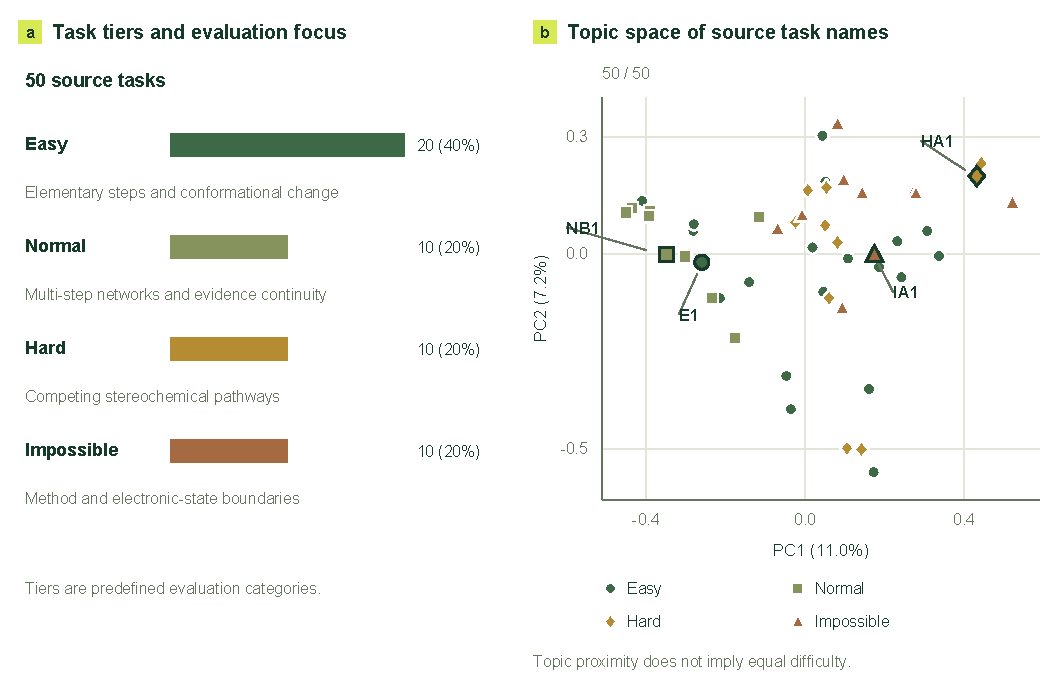
\includegraphics[width=\textwidth]{figures/fig05.pdf}
\caption{CloudraBench task composition and research themes. (a) Counts and evaluation focus of the four task tiers. (b) Two-dimensional PCA, computed with scikit-learn\citep{sklearn2011}, of BAAI/bge-m3 embeddings\citep{bgem32024} of all 50 original task names. E1, NB1, HA1, and IA1 are the four tasks used in the repeated-run experiment. Colors and marker shapes encode the predefined task tiers.}
\label{fig:05}
\end{minipage}
\end{figure*}

\subsubsection{Scoring and study configurations}

Graph structure, self-consistency, and accuracy are evaluated separately and combined with weights of 0.1, 0.3, and 0.6. Graded physical support and runtime delivery completeness are also reported. A correctly identified method limitation is scored as a supported negative conclusion. Each task lists reference-graph availability, available reference calculations, task-specific exceptions, and unresolved validation checks.

\subsubsection{Repeated-task study, primary comparison, and workflow ablations}

The repeated-task study (P1b) compares Guided, Standard, Record, and Brief-errors on E1, NB1, HA1, and IA1, with three independent runs per combination (48 task-level runs). The repeated runs used DeepSeek-v4.1-flash (1017).\citep{deepseekv42026} E1, NB1, HA1, and IA1 concern elimination preorganization, multistep decarboxylation, stereochemical ring opening, and electronic-structure method limits, respectively; their archived trajectories supply the subsequent local diagnostic cases. Its elapsed-time unit is a four-task batch at concurrency two, with three batches per configuration. The full-benchmark study (P2) retains one run for each of the 50 tasks and four configurations (200 task-level runs). All P2 configurations used DeepSeek-v4.1-flash (1017), called with the archived API alias \texttt{deepseek-v4-flash} through the official DeepSeek endpoint and streaming OpenAI-compatible chat completions, with requested minimal reasoning effort. The primary comparison is Guided against Standard using this same backbone; Standard is labelled Backbone in the figures. The P2 execution versions and request settings are listed in Supplementary Information Section S1.



Standard hides explicit DAG tools, removes enforcement of physical checks, and supplies neutral computational feedback. Guided uses the research graph, scientific checks, and detailed diagnostics. Record provides tools and records with optional physical validation; Brief-errors retains guidance while shortening diagnostics. All configurations receive the same task statements and method restrictions. The archive stores each run's code version, budget and stopping reason, together with the source files for its calculations.



Before scoring, human curators reconstruct each run's mechanism graph from its conversations, tool records, reports, and calculation files, following the agent's stated mechanistic intent and conclusions. They restore file references and record the source of each recovered field. Reconstruction uses only that run's existing calculations and conclusions. The evaluator searches its sandbox for native calculation evidence and scores the graph against Gold targets under common rules. The final dataset contains all 200 runs and reports Graph, Self-consistency, and Accuracy alongside each composite score. Paired differences and 95\% percentile intervals use 100,000 task-cluster bootstrap samples, retaining the four configurations of each task together (seed 20261031). Computational effort is measured on the 15 selected tasks with records for all four configurations, using quantum-chemical job counts and cumulative job-hours.

